%・6-2-1~3節では小窓の表示方法,あるいは顔自体の表示方法などを変更したアプリケーションを提案する

%・まず,実験用アプリケーションと同様に,

\begin{comment}
\begin{itemize}
  \item 6-2-1~3節では小窓の表示方法,あるいは顔自体の表示方法などを変更したアプリケーションを提案する
  \item まず,実験用アプリケーションと同様に,小窓に,PC使用者と,見られている参加者の2人を表示する手法を提案する
  \item 実験用アプリケーションと異なる点は以下の通り
  \item 小窓の表示位置を,球体ディスプレイの赤道部分に寄せる
  \item 顔認識ライブラリdlibを用いて,顔を認識した位置に対して小窓を表示する
  \item PC使用者は,実験用アプリケーションの時と異なり,指定の位置ではなく可変な被検者の顔の位置をクリックすることで
        被験者を見ることが出来る
  \item 顔を中心に持ってくるのではなく,GUIの空いていた領域(画面下部)にクリックした人物の顔の切り取りを表示する
  \item (dlibについての説明,アプリケーションの様子,クリックした位置に顔を持ってくるプログラムについての説明を行う)
\end{itemize}
\end{comment}

この節では,小窓にPC使用者と見られている人間の2つの顔を
表示するアプリケーションを提案する.実験用アプリケーション
との変更点は以下のとおりである.
\begin{itemize}
  \item 小窓の表示位置を,球体ディスプレイの赤道部分に寄せる
  \item 顔認識ライブラリDlib\cite{12}を用いて,顔を認識した位置に対して小窓を表示する
  \item PC使用者は,実験用アプリケーションの時と異なり,指定の位置ではなく可変な
  被験者の顔の位置をクリックすることで被検者を見ることが出来る
  \item 顔を中心に持ってくるのではなく,GUIの空いていた領域(画面下部)にクリックした人物の顔部分を表示する
\end{itemize}

変更点の1つ目は
\begin{itemize}
  \item 顔の切り抜きはもう少し下に置くことは可能か?
\end{itemize}
という,被検者からのコメントに対しての実装である.実際に,
正距円筒図法によって出力された全天球パノラマ画像に,正方形で切り取った
顔部分の画像を張り付けると,歪みを考慮していないために,上部分ほど
実際より小さく表示されてしまうという問題がある.
例えば緯度60°に相当する部分は,正距円筒図法上では赤道と同じ長さであるが
球体ディスプレイ上では赤道の長さの半分になってしまう.(表\ref{projection1}参照)よって,歪みの
影響の少ない球体ディスプレイの赤道近くに顔の小窓を表示することが適切であると
考えた.
\begin{figure}[tp]
  \centering
  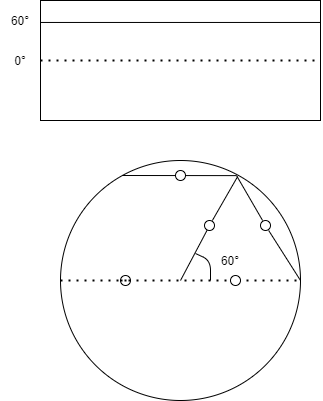
\includegraphics[scale=0.7]{fig/projection1.png}\label{projection1}
  \caption{上部分が縮小して表示される様子}
\end{figure}

変更点の4つ目は
\begin{itemize}
  \item ディスプレイのサイズ的に3人とも常に視野の中に収まってはいるので、クリックした人が真ん中に来る必要はないかな…と感じた。画像そのものが移動するよりは、クリックしている間はカーソルの周辺に枠がでる…とかのほうが「ひとりにフォーカスしている感」があって良いかもしれないと思いました。
  \item 3人のうち誰か一人を見るということが難しいと感じた(視野に全員が収まっているので誰か一人にフォーカスして話しづらい)
\end{itemize}
というプレゼンターからのコメントを反映させた.
また,顔にフォーカスし,表示させることで,全天球カメラの視野の広さによって
顔が相対的に小さく見えてしまう問題の解決も目指した.

\subsection*{Dlib}

\begin{figure}[tp]
  \centering
  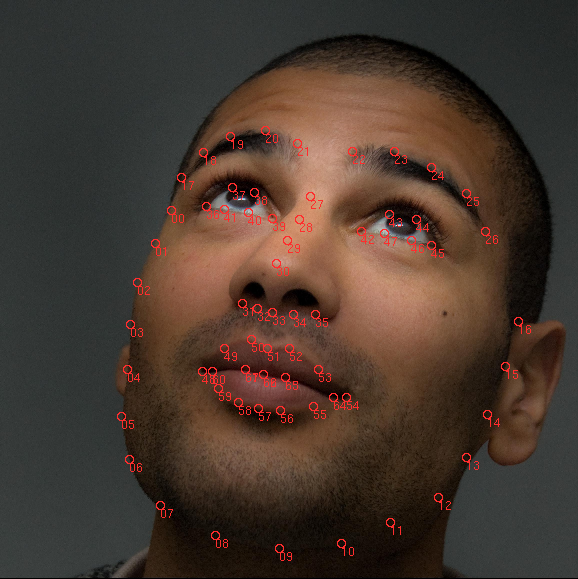
\includegraphics[scale=0.7]{fig/dlib.png}
  \caption{Dlibの顔検出} \cite{13}
\end{figure}

顔認識には,C++やpythonで利用可能な,クロスプラットフォームソフトウェアライブラリ
であるDlibを用いた.Dlibには様々な種類の顔認識モデルが事前に準備されている.
代表的なものを以下に示す.
\begin{itemize}
  \item HOG(Histograms of Oriented Gradients)+SVN(Support Vector Machine)
  \item CNN
\end{itemize}

\subsubsection*{HOG+SVN}
HOGは局所領域の輝度の勾配を
求め,ヒストグラム化した特徴量である.画像はブロックと呼ばれる局所領域
に分割され,さらにブロックはセルと呼ばれる局所領域に分割される.セル毎に
各ピクセルの輝度勾配を計算し,勾配の方向で分類したヒストグラムを作成する.
各セルの各勾配方向におけるヒストグラムは,ブロック内のヒストグラムの総和に
よって正規化される.

SVNは,データを2クラスに分類するために
最適な超平面を求めるアルゴリズムである.$n$次元空間における超平面は,
次元が$n-1$の平坦な空間であり,元の空間を2つに分割する.

\subsubsection*{CNN}
CNNは,従来のニューラルネットワークに,畳み込み層やプーリング層といった
層を組み合わせて作られるニューラルネットワークである.画像認識の分野では
よく用いられている.

\begin{figure}[tp]
  \centering
  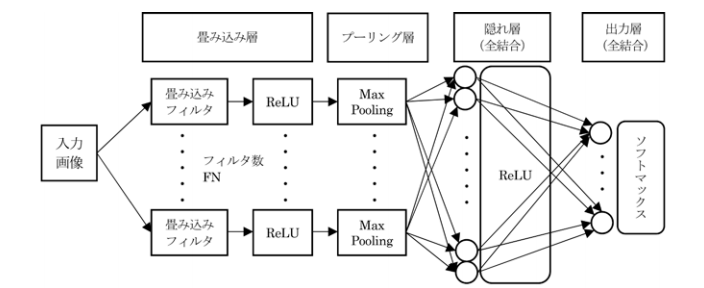
\includegraphics[scale=0.7]{fig/CNNep.png}
  \caption{CNNの一例} \cite{13}
\end{figure}

畳み込み層では,学習可能なパラメータであるカーネル及びバイアスを用いて,入力に対して
畳み込みが行われる.画像データの畳み込みに際しては,ある注目ピクセルと
その周辺のピクセルが出力に用いられることで,画像の空間的な情報が損なわれにくい
という利点がある.

カーネル$K$のサイズが$N*N$であった場合,画像のあるピクセルの周辺$K*K$サイズの
領域$A$にカーネルを適用した結果は,$K$と$A$のアダマール積となる.すなわち

\begin{eqnarray}
  \sum_{i=1}^{N} \sum_{j=1}^{N} k_{ij}a_{ij} \nonumber 
\end{eqnarray}
である.

カーネルを適用する領域は通常1ピクセルずつずらされる.そうして
全ての領域にカーネルが適用され,バイアスを加算した結果が畳み込み層の出力
として用いられる.

\begin{figure}[tp]
  \centering
  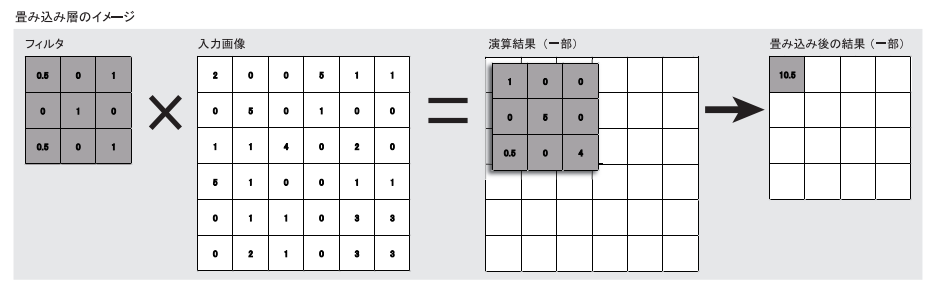
\includegraphics[scale=0.6]{fig/conv.png}
  \caption{畳み込みのイメージ} \cite{14}
\end{figure}

プーリング層は,通常畳み込み層の直後の層であり,畳み込み層の
出力を,カーネルを用いてダウンサンプリングした結果を出力する.

ここで用いられるカーネルは,カーネル適用範囲の平均値を出力するものと,
カーネル適用範囲の最大値を出力するものがよく用いられている.
前者の場合はAverage Pooling層と呼ばれ,後者ならMax Pooling層と呼ばれる.
カーネルの適用範囲のずらし幅はストライドと呼ばれ,様々な値が設定されている.

\begin{figure}[tp]
  \centering
  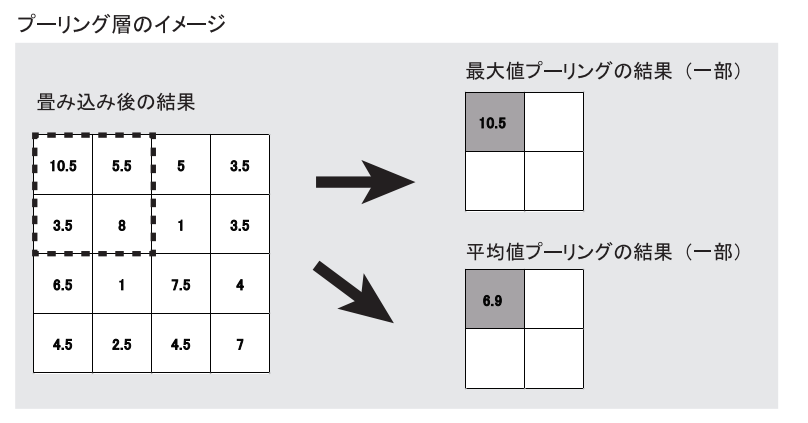
\includegraphics[scale=0.7]{fig/pooling.png}
  \caption{プーリングのイメージ} \cite{14}
\end{figure}

今回のアプリケーションでは,より精度の高いCNNを用いたモデルを使用した.
一方で,HOG+SVNを用いるモデルは,識別実行速度が速いという利点がある.





